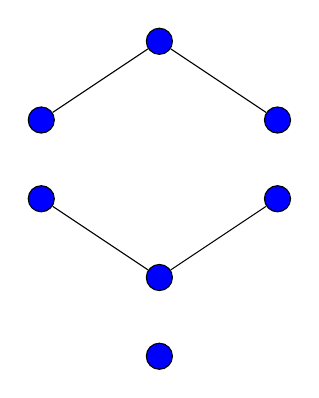
\begin{tikzpicture}[x=1.5cm,y=1cm,every node/.style={draw,solid,shape=circle,fill=blue}]

  % Specification of nodes (position, etc.)
  \node (a0) at (0,0) {};
  \node (b0) at (-1,-1) {};
  \node (b1) at (1,-1) {};
  \node (g0) at (-1,-2) {};
  \node (g1) at (1,-2) {};
  \node (j) at (0,-3) {};
  \node (c) at (0,-4) {};

  \begin{scope}[-]
    \tikzstyle{every node}=[draw,below]
    \draw[solid] (a0) to (b0);
    \draw[solid] (a0) to (b1);
    \draw[solid] (g0) to (j);
    \draw[solid] (g1) to (j);
  \end{scope}

\end{tikzpicture}
